\documentclass{article}
% [landscape]
\usepackage{amsmath, amsthm, amssymb, bm, color, framed, graphicx, hyperref, mathrsfs}
\usepackage{graphicx}%图片头文件
\usepackage{float} %指定图片位置
\usepackage{subfigure}%并排子图 共享标题 有子标题
\usepackage{caption}
\usepackage[margin=1in,letterpaper]{geometry} 

% code
\usepackage{listings} 
\usepackage{xcolor}
\lstset{
  language=Matlab,  %代码语言使用的是matlab
  frame=shadowbox, %把代码用带有阴影的框圈起来
  rulesepcolor=\color{red!20!green!20!blue!20},%代码块边框为淡青色
  keywordstyle=\color{blue!90}\bfseries, %代码关键字的颜色为蓝色,粗体
  commentstyle=\color{red!10!gray!70}\textit,    % 设置代码注释的颜色
  showstringspaces=false,%不显示代码字符串中间的空格标记
  numbers=left, % 显示行号
  numberstyle=\tiny,    % 行号字体
  stringstyle=\ttfamily, % 代码字符串的特殊格式
  breaklines=true, %对过长的代码自动换行
  extendedchars=false,  %解决代码跨页时,章节标题,页眉等汉字不显示的问题
%   escapebegin=\begin{CJK*},escapeend=\end{CJK*},      % 代码中出现中文必须加上,否则报错
  texcl=true}


\usepackage{ctex}
\usepackage{amsmath}
\usepackage{graphicx}
\usepackage{epstopdf}
\usepackage{tikz}
\usepackage{psfrag}
\usepackage{natbib}
\usepackage{hyperref}

% \begin{document}

\renewcommand{\refname}{参考文献}
\renewcommand{\figurename}{图}
\renewcommand{\abstractname}{摘要}
\title{《磁流体力学的数值模拟方法》-第3次作业\footnote{2022 春季《磁流体力学的数值模拟方法》}}

\author{苏镇波\footnote{Email: zbsu@mail.ustc.edu.cn, 学号: SA21022002}
\and
康樨\footnote{Email: kx\_0045@mail.ustc.edu.cn, 学号: SA21007083}
\and
蓝翔\footnote{Email: shsxjujishou@163.com, 学号: SA21214038}
}

\date{%
\scriptsize%
%CAS Key Laboratory for Basic Plasma Physics, School of Earth and Space Sciences,
%\\
%University of Science and Technology of China, Hefei, Anhui 230026, China
中国科学技术大学物理学院天文系,合肥 230026\\
中国科学技术大学地球与空间科学学院, 合肥 230026\\
中国科学技术大学核科学技术学院, 合肥 230026
%
}

\begin{document}
\maketitle

\begin{abstract}
针对一维激波管问题在一定初值条件下对其中的密度、质量流及能量的空间分布随时间的演化过程进行了数值模拟和解析求解。我们讨论了解析解的物理特性及数值解的数值特性并比较了解析解和数值解的差异。
\end{abstract}

\section{引言}
一维激波管问题是典型的一维可压缩无粘气体动力学问题。激波管是一根两端封闭、内部充满气体的直管。在直管中由一薄膜隔开两部分密度、压力不同的气体。在初始时刻薄膜破裂,气体从高压段冲向低压端,同时在管内形成激波、稀疏波及接触间断等复杂波系。
\par
我们对这个问题主要采取了Roe、Upwind守恒型及非守恒型格式进行数值求解同时也求得了理论解进行对比,以分析理论解所代表的实际物理特性和数值解代表的数值格式特性并对比理论解与数值解的差异。

\section{方程及数值方法}

粒子数守恒方程、动量守恒方程及能量守恒方程可统一写成如下形式:
\begin{equation} 
{\partial w\over\partial t}+{\partial f(w)\over\partial x}=0 \label{con:Euler}
\end{equation}

\begin{align}
w(x,t)|_{t=0} = \left\{ \begin{array}{ll}
W_L, & \quad x < 0 \\
W_R, & \quad x > 0
\end{array} \right.
\end{align}
其中
\begin{align}
w =& \left[\begin{array}{c}
\rho\\
m\\
E
\end{array}\right],
\\
f(w) =& u w + \left[\begin{array}{c}
0\\
p\\
p u
\end{array}\right] = \left[\begin{array}{c}
m
\\
(\gamma - 1) E + \frac{3 - \gamma}{2} \frac{m^2}{\rho}
\\
(\gamma E - \frac{\gamma - 1}{2} \frac{m^2}{\rho}) \frac{m}{\rho}
\end{array}\right],
\\
m =& \rho u,
\\
p =& (\gamma - 1)(E - \frac{1}{2} \rho u^2).
\end{align}
这里, $\rho$, $u$, $p$ 和 $E$ 分别是密度, 速度, 压力和总能量. 
\par
\subsection{Roe 格式}
对于Roe格式, 式(\ref{con:Euler})可写为:
\begin{align}
\frac{\partial W}{\partial t} + A_{j+1/2} \frac{\partial W}{\partial x} = 0,
\end{align}
根据\cite{danaila2007}书中第10章 (10.60) 式,有:
\begin{align}
W_j^{n+1} =& W_j^n - \frac{\Delta t}{\Delta x} (\Phi(W^n_j,W_{j+1}^n)-\Phi(W^n_j, W^n_{j-1})
\end{align}
其中,$\Phi(W^n_j, W^n_{j+1})=\frac{1}{2}\{{F(W^n_j)+F(W^n_{j+1})-|A|_{j+1/2}[W^n_{j+1}-W^n_j]}\}$.

其中 $A = \frac{\partial F}{\partial u}$, $A$ 的表达式如下
\begin{align*}
A =& \frac{\partial f}{\partial w} = \left[\begin{array}{ccc} 0 & 1 & 0
\\
\frac{1}{2} (\gamma  - 3) u^2 & -(\gamma - 3) u & \gamma - 1
\\
(\gamma - 1) u^3 - \gamma \frac{u}{\rho} E & \gamma \frac{1}{\rho} E-\frac{3}{2} (\gamma
- 1) u^2 & \gamma u
\end{array}
\right]
\end{align*}
\par
矩阵A的特征值为:$\lambda_1=u-c, \lambda_2=u, \lambda_3=u+c$,
对应的特征向量为:
\begin{align}
e_1=  \left[\begin{array}{c}1\\ u-a\\ H-ua\end{array}\right], \qquad e_2 = \left[\begin{array}{c}1 & u & \frac{1}{2}u^2\end{array}\right], \qquad e_3=\left[\begin{array}{c} 1 & u+a & H+ua\end{array}\right]
\end{align}
其中,$H$为总比焓:
\begin{align}
    H=\frac{H+p}{\rho}=\frac{a^2}{\gamma-1}+\frac{1}{2}u^2
\end{align}
因此,我们得到了关于Roe格式平均的计算方式:
\begin{align}
    \bar{\rho}=[(\sqrt{\rho_L}+\sqrt{\rho_R})/2]^2 
\end{align}    
\begin{align}
    \bar{u} = (\sqrt{\rho_L}u_L+\sqrt{\rho_R}u_R)/(\sqrt{\rho_L}+\sqrt{\rho_R})
\end{align}
\begin{align}
    \bar{H} = (\sqrt{\rho_R}H_L+\sqrt{\rho_R}H_R)/(\sqrt{\rho_L}+\sqrt{\rho_R})
\end{align}
其中,下标$L, R$分别为激波管区域的左区和右区,激波管区域划分详见\cite{danaila2007}第十章图10.1。
\subsection{Upwind 格式}
对应的Upwind非守恒型:式(\ref{con:Euler})可写为
\begin{align}
\frac{\partial U}{\partial t} + A \frac{\partial U}{\partial x} = 0,
\end{align}
其中
\begin{align}
U = [u_j] = \left[\begin{array}{c}\rho\\ u\\ p\end{array}\right], \qquad A = A_{ij} = \left[\begin{array}{ccc}u & \rho & 0\\
0 & u & 1/\rho\\ 0 & \gamma p & u\end{array}\right]
\end{align}
矩阵 $A$ 的特征值为 $u-a$, $u$, $u+a$ ($a^2 = \gamma p/\rho$), 对应的左右特征向量矩阵为 $L$ 和 $R$ 写为
\begin{align}
L =& [L_{ij}] = \left[\begin{array}{ccc}0 & -\rho a & 1\\ a^2 & 0 & -1\\ 0 & \rho a & 1\end{array}\right],
\\
R =& [R_{ij}] = \left[\begin{array}{ccc}\frac{1}{2a^2} & \frac{1}{a^2} & \frac{1}{2a^2}\\
-\frac{1}{2\rho a} & 0 & \frac{1}{2\rho a}\\ \frac{1}{2} & 0 & \frac{1}{2}\end{array}\right]
\end{align}
\par
更进一步可写为:
\begin{align}
\frac{\partial u_k}{\partial t} + \sum_i \sum_j \left\{R_{ki} \lambda_i L_{ij} \frac{\partial
u_j}{\partial x}\right\} = 0\label{con:next}
\end{align}
\par
对应的Upwind守恒型:
矩阵$A$ 的表达式变为
\begin{align*}
A =& \frac{\partial f}{\partial w} = \left[\begin{array}{ccc} 0 & 1 & 0
\\
\frac{1}{2} (\gamma  - 3) u^2 & -(\gamma - 3) u & \gamma - 1
\\
(\gamma - 1) u^3 - \gamma \frac{u}{\rho} E & \gamma \frac{1}{\rho} E-\frac{3}{2} (\gamma
- 1) u^2 & \gamma u
\end{array}
\right]
\end{align*}
可求得此时矩阵A对应的左右特征向量矩阵。


\section{解析、数值结果及讨论}
\subsection{Roe 格式}
我们选取了初值条件:
\begin{align}
    W_L = \left[\begin{array}{l}
    0.445\\
    0.311\\
    8.928
    \end{array}\right], \quad W_R = \left[\begin{array}{l}
    0.5\\
    0\\
    1.4275
    \end{array}\right]
\end{align}
空间范围位于-1=<x<=1内、时间位于t=0.14时的结果作分析($\gamma=1.4$)。对于解析求解的结果(见图\ref{fig:Roe}灰色虚线结果),可以清楚地看到存在三种不同相速度的波模。其中x=0.347处存在代表了激波的间断,该间断两侧密度、速度及压力均发生突变,其相速度$v_{\phi}$=u+a=2.480;x=0.214处存在接触间断,该间断两侧密度发生突变而速度、压力均连续,相速度$v_{\phi}$=u-a=1.529;在x=-0.229和-0.369处存在弱间断特征,在两点附近密度、速度及压力数值连续但一阶导数不连续,两处相速度$v_{\phi}$=u分别为-1.636和-2.633。
\par
对于Roe格式下的数值计算,我们取网格数 256,Courant-Friedrichs-Lewy (CFL) 系数 0.5,根据\cite{danaila2007}一书中10.2.2节的解析解的描述, 以及10.3.2节对Roe格式数值解的描述, 可得到如下图示结果:
\begin{figure}[H]
\centering
\includegraphics[width=0.8\textwidth]{Roe.pdf}
\caption{从上到下:第一幅图为密度;第二幅图为质量流m的空间分布;第三幅图为能量的空间分布。其中灰色虚线是t=0.14时刻的精确解,黑色实线是 t=0.14 时 Roe 格式的空
间分布。}
\label{fig:Roe}
\end{figure}
\par
对Roe格式的数值计算分析:由于Roe格式的缺陷,其在拐点处 (间断点) 处会震荡得厉害,但是由于耗散比较厉害,粘性过大,间断处的数值格式表现出了连续的性质。对于x=0.347处,波传播速度为2.1552(速度值为正代表波自左向右传播,为负代表波自右向左传播);对于x=0.214处,波的传播速度为1.5018;对于x=-0.229和-0.369处,波传播速度分别为-1.9122和-2.4781。

后续的工作中,可进行分析不同网格、不同CFL系数时,Roe数值格式解的变化。
\par
\subsection{Upwind 格式}
对于Upwind的守恒型格式下的数值计算,我们取网格数263,Courant系数0.0875,在时刻t=0.14时,得到如图\ref{fig:upwind1} 所示各物理量的空间分布结果:
\begin{figure}[H]
\centering
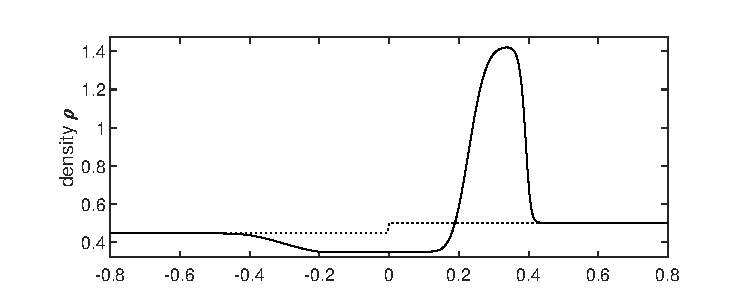
\includegraphics[width=0.8\textwidth]{Upwind_con_d.eps}
\includegraphics[width=0.8\textwidth]{Upwind_con_m.eps}
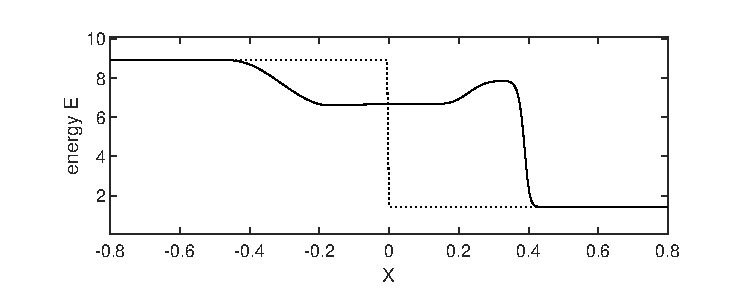
\includegraphics[width=0.8\textwidth]{Upwind_con_e.eps}
\caption{从上到下:第一幅图为密度\rho的空间分布;第二幅图为质量流m的空间分布;第三幅图为能量的空间分布。其中虚线是初始时刻的分布,实线是t=0.14时Upwind的守恒型格式的数值计算的空间分布。}
\label{fig:upwind1}
\end{figure}
对Upwind的守恒型格式的数值计算分析:数值解中在一定区域内也有类似间断的现象产生,但由于耗散等原因,间断表现出了连续的性质。对于x=0.347处,波传播速度为2.1540(速度值为正代表波自左向右传播,为负代表波自右向左传播);对于x=0.214处,波的传播速度为1.4988;对于x=-0.229和-0.369处,波传播速度分别为-1.8066和-2.4637。
\par

对于Upwind的非守恒型格式下的数值计算,我们取网格数263,Courant系数0.0875,在时刻t=0.14时,得到如图\ref{fig:upwind2}所示各物理量的空间分布结果:
\begin{figure}[H]
\centering
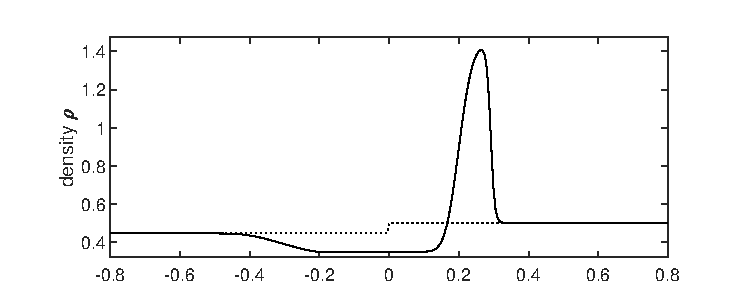
\includegraphics[width=0.8\textwidth]{Upwind_non_con_d.eps}
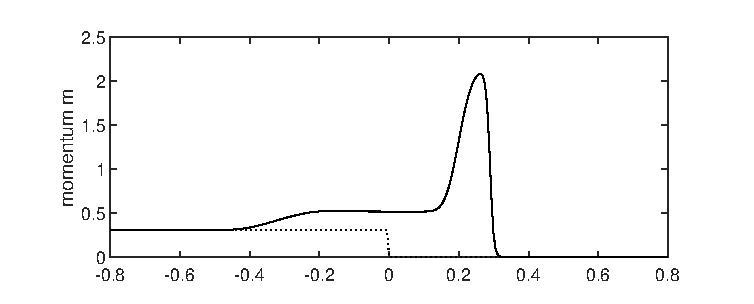
\includegraphics[width=0.8\textwidth]{Upwind_non_con_m.eps}
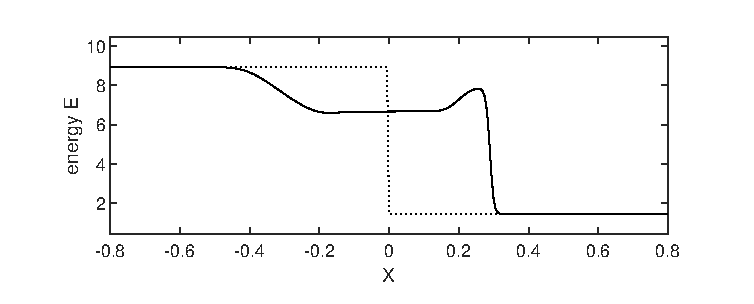
\includegraphics[width=0.8\textwidth]{Upwind_non_con_e.eps}
\caption{从上到下:第一幅图为密度\rho的空间分布;第二幅图为质量流m的空间分布;第三幅图为能量的空间分布。其中虚线是初始时刻的分布,实线是t=0.14时Upwind的非守恒型格式的数值计算的空间分布。}
\label{fig:upwind2}
\end{figure}
对Upwind的非守恒型格式的数值计算分析:对于x=0.347处,波传播速度为1.2667远低于解析解,这也带来非守恒型格式的峰处半高宽长度要低于解析解的激波——接触间断间的平台长度。该结果是非守恒型格式的固有缺陷,即便加密时空网格也无法改观;对于x=0.214处,波的传播速度为1.4792;对于x=-0.229和-0.369处,波传播速度分别为-1.7946和-2.4517。
\section{分工说明}
苏镇波负责了Roe格式的数值计算及分析,蓝翔负责了Upwind格式的数值计算及分析,苏镇波、康樨、蓝翔负责了 \LaTeX\xspace 的整理与排版。

\section{附件}
\begin{enumerate}
\item
MHD\_Group10\_hw3.tex-本报告 \LaTeX\xspace 文件
\item
MHD\_Group10\_hw3.pdf-本报告PDF输出文件
\item
code\_combination.txt-图\ref{fig:Roe},\ref{fig:upwind1}和\ref{fig:upwind2}对应的Python,Matlab计算和绘制代码
\item
Roe.pdf-图\ref{fig:Roe}的pdf文件,由Python绘制
\item
Upwind\_con\_d.eps-图\ref{fig:upwind1}的eps文件,由Matlab绘制
\item 
Upwind\_con\_m.eps-图\ref{fig:upwind1}的eps文件,由Matlab绘制
\item
Upwind\_con\_e.eps-图\ref{fig:upwind1}的eps文件,由Matlab绘制
\item
Upwind\_non\_con\_d.eps-图\ref{fig:upwind2}的eps文件,由Matlab绘制
\item 
Upwind\_non\_con\_m.eps-图\ref{fig:upwind2}的eps文件,由Matlab绘制
\item
Upwind\_non\_con\_e.eps-图\ref{fig:upwind2}的eps文件,由Matlab绘制
\item
References.bib-本报告的参考文献
\end{enumerate}

\bibliographystyle{apalike}
\bibliography{References}

\end{document}


